\documentclass{article}
\usepackage{amsmath}
\usepackage{amssymb}
\usepackage{graphicx}
\usepackage{hyperref}
\usepackage[version=4]{mhchem}


\begin{document}
\section*{Problem}
In \(\triangle A B C, A M\) is the median. \(A T\) is the angle bisector of \(\angle A . B E \perp A T\) at \(T\) and \(C F \perp A T\) at \(F\). Show that \(M E=M F\).\\
\centering
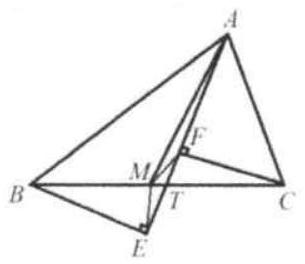
\includegraphics[width=\textwidth]{images/065(1).jpg}

\section*{Solution}
Method 1:\\
Extend \(C F\) to meet \(A B\) at \(C^{\prime}\).\\
Since \(A T\) is the angle bisector of \(\angle A, A F\) is the angle bisector of \(\angle A . A F\) is the perpendicular bisector of \(C^{\prime} C\) in \(\triangle A C^{\prime} C\), so \(\triangle A C^{\prime} F \cong \triangle A C F, C F=F C^{\prime}\).

Since \(F\) is the midpoint of \(C C^{\prime}, M\) is the midpoint of \(B C\), \(F M / / B C^{\prime} / / A B . \angle M F E=\angle B A T\).\\
Extend \(B E\) to meet the extension of \(A C\) at \(E^{\prime}\).\\
\centering
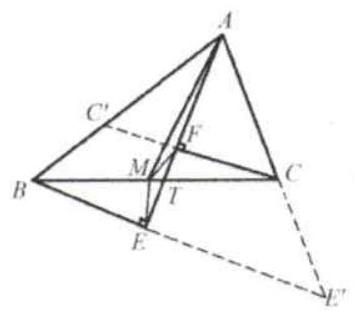
\includegraphics[width=\textwidth]{images/068(1).jpg}


Similarly, we get \(M E / / C E \prime, \angle M E F=\angle C A T\).\\
Since \(\angle B A T=\angle C A T, \angle M F E=\angle M E F\). Thus \(M E=M F\).

Method 2:\\
Extend \(C F\) to meet \(A B\) at \(C^{\prime}\).\\
Since \(A T\) is the angle bisector of \(\angle A, A F\) is the angle bisector of \(\angle A . A F\) is the perpendicular bisector of \(C^{\prime} C\) in \(\triangle A C^{\prime} C\), so \(\triangle A C^{\prime} F \cong \triangle A C F, C F=F C^{\prime}\).\\
Since \(F\) is the midpoint of \(C C^{\prime}, M\) is the midpoint of \(B C\), \(M F=\frac{1}{2} B C\).\\
\centering
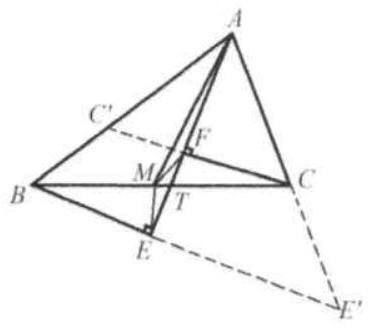
\includegraphics[width=\textwidth]{images/069.jpg}

Extend \(B E\) to meet the extension of \(A C\) at \(E^{\prime}\).\\
Similarly, we get \(M E=\frac{1}{2} C E\).\\
Since \(C C^{\prime} / / B E^{\prime}, C B=C E^{\prime}\). Thus \(M E=M F\).

\end{document}
